%%%%%%%%%%%%%%%%%%%%%%%%%%%%%%%%%%%%%%%%%%%%%%%%%%%%%%%%%%%%%%%%%%%%%%%%%%%%%%%
%  X-Road Colombia: An Automated Maturity Assessment Platform for
%  Public-Sector Interoperability
%
%  VERSION COMPACTA (objetivo: maximo 12 paginas) -- formato Springer LNCS.
%  La version extensa (20 paginas) esta en articulo_xroad.tex
%
%  Compilar con:
%      pdflatex articulo_xroad_12p.tex
%      pdflatex articulo_xroad_12p.tex
%%%%%%%%%%%%%%%%%%%%%%%%%%%%%%%%%%%%%%%%%%%%%%%%%%%%%%%%%%%%%%%%%%%%%%%%%%%%%%%
\documentclass[runningheads]{llncs}

\usepackage[T1]{fontenc}
\usepackage[utf8]{inputenc}
\usepackage{graphicx}
\usepackage{booktabs}
\usepackage{amsmath}
\usepackage{amssymb}
\usepackage{url}
\usepackage{tikz}
\usetikzlibrary{arrows.meta,positioning}
\usepackage[hidelinks]{hyperref}

\pagestyle{headings}

% --- Revision ciega: autores omitidos (igual que el documento de referencia).
% --- Descomente el bloque real cuando el articulo deje de estar anonimizado.
\author{Author(s) omitted for blind review}
\institute{Institution omitted for blind review}
%
% \author{Esteban Lopez Usma}
% \institute{Programa de Administraci\'on de Sistemas Inform\'aticos\\
%            \email{elopezu@unal.edu.co}}

\begin{document}

\title{X-Road Colombia: An Automated Maturity Assessment Platform for
Public-Sector Interoperability}

\titlerunning{X-Road Colombia: Automated Maturity Assessment}
\authorrunning{Omitted for blind review}

\maketitle

\begin{abstract}
This paper presents \emph{X-Road Colombia}, a full-stack platform that
automates the diagnosis of digital interoperability maturity in the
Colombian public sector. Colombia adopted X-Road as the backbone of its
interoperability layer and defined, through MinTIC, a framework structured
in four domains: legal, organizational, semantic, and technical. No
independent instrument currently contrasts administrative registration with
verifiable operational capability. The platform operationalizes the MinTIC
framework into measurable indicators computed over a registry of entities,
their published services, and their declared X-Road state, combining a
deterministic maturity engine, HTTP-based API introspection, semantic
validation, gap analysis, clustering and prediction models, geospatial and
network visualizations, and multi-format reporting behind a hardened REST
API. The diagnostic over 127 registered entities yields a national maturity
index of 2.3/5.0 (SD = 1.1), a \emph{Basic} level, with the technical domain
leading (3.1) and the semantic domain weakest (1.9). The study exposes a
registration--operation gap: 32\% of the registered entities remain at the
initial level, and the Hacienda y Finanzas sector concentrates the highest
maturity (3.8). An automatic cross-check reproduces the same domain ordering
(semantic 45.3, organizational 49.3, legal 55.7, technical 58.3 on a 0--100
scale). Results indicate that evidence-based automated auditing is feasible
and that connectivity alone does not produce interoperability.

\keywords{Interoperability \and X-Road \and Digital government \and
Maturity model \and Automated assessment \and Colombia}
\end{abstract}

\section{Introduction}
\label{sec:intro}

Colombia has prioritized state modernization as a cross-cutting public
policy objective, materialized in a digital transformation agenda and in
normative instruments that mandate transparency, open data, and efficient
public service delivery \cite{conpes3975,ley1712,decreto1078}. Within that
agenda, digital interoperability is a foundational capability: the
organizational and technological condition that allows heterogeneous public
institutions to exchange information securely, timely, and with a shared
meaning, so that citizens are not asked for data the State already holds.

The country adopted X-Road as the interoperability backbone of the State and
defined, through MinTIC, an \emph{Interoperability Framework for Digital
Government} organized in four domains---legal, organizational, semantic, and
technical \cite{mintic2025}. X-Road is a distributed data-exchange layer in
which each organization runs a security server that publishes and consumes
services through machine-processable contracts and signed messages
\cite{niis2026}; its operational inventory is coordinated by the National
Digital Agency (AND) \cite{and2025}. Despite this architecture,
implementation has progressed unevenly: some entities expose integrated,
documented services while many others remain at early digitalization stages.
More importantly, the symptoms of that asymmetry---duplicated data requests,
routing errors, undetected service failures---cannot be diagnosed with the
information that is publicly available, because administrative registration
in a catalog is not the same as operational interoperability.

This work addresses the absence of an \emph{independent, automated, and
replicable} instrument that measures entity maturity against the national
framework, contrasts registration with verifiable service availability,
localizes the domains and sectors where deficits concentrate, and produces
traceable evidence for prioritization. Manual reviews and self-declaration
instruments are insufficient: they are costly, hard to repeat, and
systematically overestimate readiness. The remainder of this paper reviews
the conceptual framework (Section~\ref{sec:related}), the architecture
(Section~\ref{sec:arch}), the implementation (Section~\ref{sec:impl}), the
evaluation (Section~\ref{sec:eval}), the security and governance model
(Section~\ref{sec:security}), and the conclusions
(Section~\ref{sec:conclusions}).

\paragraph{Contributions.} (i)~An operational model translating the four
MinTIC domains into measurable indicators; (ii)~a deterministic maturity
engine with an explicit rubric and ordinal levels that removes subjective
valuation; (iii)~a software instrument that verifies evidence automatically
through API introspection, semantic validation, and severity-ranked gap
analysis; (iv)~a visual analytics layer---geospatial map, service matrix, and
relationship graph---that exposes the state interconnection map; and (v)~a
reproducible engineering blueprint, deployable with one Docker Compose
command and hardened with authentication, authorization, and auditing.

\paragraph{Research questions.} RQ1: what is the interoperability maturity
level of the entities registered in the national X-Road node when measured
against the MinTIC framework? RQ2: what gap exists between formal
registration and verifiable operational service availability? RQ3: which
domains concentrate the largest deficits? RQ4: can an automated assessment
instrument improve decision-making compared with administrative
self-reporting?

\section{Conceptual Framework and Related Work}
\label{sec:related}

\begin{sloppypar}
Interoperability is the capability of heterogeneous organizations to
exchange information for mutually beneficial goals \cite{eif2017}. In the
public sector it is broader than connectivity: it requires coordinated
processes, harmonized legal conditions, and aligned data meaning. The
reference frameworks converge on a four-layer decomposition---legal,
organizational, semantic, and technical---which means that two institutions
can be physically connected and still be unable to produce a legally valid,
semantically correct, and operationally useful exchange. The semantic layer
is the most fragile: without shared dictionaries, code lists, and canonical
schemas, each pair of entities must negotiate bilateral mappings, which does
not scale and silently degrades data quality.
\end{sloppypar}

\begin{sloppypar}
MinTIC's framework defines the reference architecture, standards, and
governance mechanisms for public data exchange \cite{mintic2025} and
organizes assessment into four domains: \emph{legal} (normative basis and
lawful processing), \emph{organizational} (governance, roles, and
processes), \emph{semantic} (shared meaning, metadata, and vocabularies),
and \emph{technical} (connectivity, security, API quality, and non-functional
attributes). On top of the domains it defines a staged maturity progression.
The platform operationalizes four computable levels---\emph{Inicial},
\emph{B\'asico}, \emph{Intermedio}, and \emph{Avanzado}
(Section~\ref{sec:arch:engine})---and the diagnostic of
Section~\ref{sec:eval} additionally uses a normalized 1--5 index.
\end{sloppypar}

X-Road, maintained by the Nordic Institute for Interoperability Solutions
\cite{niis2026}, is member-centric: each organization registers with a member
class and code and deploys security servers that publish and consume
services. Because data stays in the source systems and moves through
authenticated, signed, and logged transactions, X-Road became the backbone of
several national architectures, including Colombia's. For diagnostic
purposes, however, the member registry is insufficient: being
\emph{registered} proves enrollment, not that the entity publishes a
documented, reachable, and consumable service.

Maturity models structure evolutionary capability paths. De Bruin et al.
\cite{debruin2005} formalized their design phases and Becker et al.
\cite{becker2009} established design principles for IT management maturity
models; in electronic government, recent work surveys the landscape of
e-government maturity models \cite{okan2024} and addresses
cross-organizational data interoperability maturity \cite{wahyuni2024}. Three
limitations persist: instruments are usually \emph{self-declared} (upward
bias), \emph{manual} (expensive to repeat), and \emph{static}
(disconnected from artifacts that change continuously). This work inverts the
evidence flow: the platform computes the level from artifacts and observable
attributes instead of asking entities to declare it. Consequently, the gap
addressed here is the shortage of open, automated, and reproducible
instruments that measure interoperability maturity from verifiable evidence
in a specific national regulatory context. Table~\ref{tab:comparison}
positions the approach against the dominant alternatives.

\begin{table}[t]
\caption{Comparison of approaches for public-sector interoperability
assessment across functional dimensions.}
\label{tab:comparison}
\centering
\setlength{\tabcolsep}{3pt}
\scriptsize
\begin{tabular}{p{4.3cm}ccccc}
\toprule
Approach & Evidence & Auto. & Multi- & Service & Ecosys. \\
         & based    & scoring & domain & verification & visual. \\
\midrule
Administrative self-reporting & No & No & Partial & No & No \\
Static BI dashboard on registry & Partial & No & No & No & Partial \\
Manual maturity survey / expert panel & Partial & No & Yes & No & No \\
Technical monitoring of exchange layer & Yes & Yes & No & Yes & Partial \\
\textbf{Proposed platform} & Yes & Yes & Yes & Yes & Yes \\
\bottomrule
\end{tabular}
\end{table}

\section{System Architecture}
\label{sec:arch}

The platform is a decoupled three-tier client--server system
(Fig.~\ref{fig:architecture}): a single-page application for visualization
and interaction, a REST API that concentrates business logic and assessment,
and a relational persistence tier, all orchestrated with Docker and
communicating exclusively through the HTTP contract. Three design decisions
shape it. The \emph{scoring rules are deterministic and explicit}, so every
point is attributable to a named indicator and a result can be audited.
\emph{Evidence is stored next to the result}, since each assessment keeps its
domain scores, criteria, assessor, date, and recommendations, enabling
historical comparison. And \emph{verification is separated from
visualization}: connectors and analyzers produce evidence, the maturity
engine converts it into scores, and the interface consumes aggregated
results.

\begin{figure}[t]
\centering
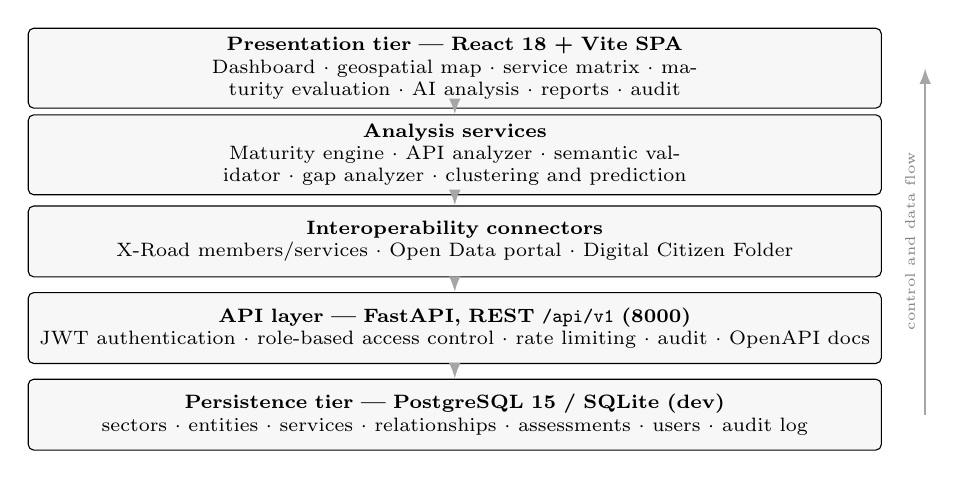
\begin{tikzpicture}[
    font=\scriptsize,
    layer/.style={draw, rounded corners=2pt, text width=10.6cm,
                  minimum height=0.9cm, align=center, fill=gray!6},
    flow/.style={-{Latex[length=2mm]}, draw, gray!70, thick}
]
\node[layer] (l5) at (0,4.6)
  {\textbf{Presentation tier --- React 18 + Vite SPA}\\
   Dashboard $\cdot$ geospatial map $\cdot$ service matrix $\cdot$ maturity
   evaluation $\cdot$ AI analysis $\cdot$ reports $\cdot$ audit};
\node[layer] (l4) at (0,3.5)
  {\textbf{Analysis services}\\
   Maturity engine $\cdot$ API analyzer $\cdot$ semantic validator $\cdot$
   gap analyzer $\cdot$ clustering and prediction};
\node[layer] (l3) at (0,2.4)
  {\textbf{Interoperability connectors}\\
   X-Road members/services $\cdot$ Open Data portal $\cdot$ Digital Citizen
   Folder};
\node[layer] (l2) at (0,1.3)
  {\textbf{API layer --- FastAPI, REST \texttt{/api/v1} (8000)}\\
   JWT authentication $\cdot$ role-based access control $\cdot$ rate limiting
   $\cdot$ audit $\cdot$ OpenAPI docs};
\node[layer] (l1) at (0,0.2)
  {\textbf{Persistence tier --- PostgreSQL 15 / SQLite (dev)}\\
   sectors $\cdot$ entities $\cdot$ services $\cdot$ relationships $\cdot$
   assessments $\cdot$ users $\cdot$ audit log};
\draw[flow] (l5) -- (l4);
\draw[flow] (l4) -- (l3);
\draw[flow] (l3) -- (l2);
\draw[flow] (l2) -- (l1);
\draw[flow] ([xshift=0.55cm]l1.east) -- ([xshift=0.55cm]l5.east)
  node[midway, above, rotate=90, font=\tiny, text=gray] {control and data flow};
\end{tikzpicture}
\caption{Layered architecture of the proposed platform. Arrows indicate the
control and data flow between tiers.}
\label{fig:architecture}
\end{figure}

\paragraph{Data model.} The schema has seven tables. \emph{Sector} groups
entities by domain of public action. \emph{Entity} stores identity (name,
acronym, NIT, sector), territorial location (department, municipality,
coordinates), contact channels, the X-Road state
(\texttt{not\_connected}, \texttt{pending}, \texttt{connected}, with member
code and connection date), and the CIO contact fields used for fieldwork.
\emph{Service} describes what is published: category, protocol
(\texttt{REST}, \texttt{SOAP}, \texttt{X-Road}), endpoint URL, API version,
declared data, semantic and security standards, status, and documentation
URL. \emph{Relationship} models the directed exchange between a source and a
target entity with its protocol and state, and is the substrate of the
ecosystem graph. \emph{MaturityAssessment} stores, per entity and date, the
global level and score, the four domain scores, six detailed criteria, the
assessor, and the recommendations. Finally, \emph{Usuario} and
\emph{Auditoria} support authentication and traceability. Because the X-Road
state is a first-class attribute, the registration--operation gap is computed
directly as a query, and because assessments are append-only, the evolution
of an entity can be reconstructed.

\subsection{The Maturity Assessment Engine}
\label{sec:arch:engine}

The engine converts attributes and evidence into a composite score
$S \in [0,100]$ and an ordinal level, using an explicit rubric:

\begin{equation}
S = 25\,s_{\text{xroad}} + 25\,s_{\text{services}} + 20\,s_{\text{contact}}
    + 15\,s_{\text{sector}} + 15\,s_{\text{geo}}
\label{eq:score}
\end{equation}

where $s_{\text{xroad}} = 1$ if the entity is connected to X-Road and $0.4$
if the connection is pending; $s_{\text{services}} = \min(n/4, 1)$ with $n$
the number of published services; $s_{\text{contact}}$ is the weighted
presence of website, email, and phone; $s_{\text{sector}} = 1$ if the entity
is classified in a sector; and $s_{\text{geo}} = 1$ if valid coordinates are
registered. The level follows thresholds: \emph{Inicial} for $S < 25$,
\emph{B\'asico} for $25 \le S < 50$, \emph{Intermedio} for $50 \le S < 75$,
and \emph{Avanzado} for $S \ge 75$. In parallel, the engine derives the four
MinTIC domain scores from the same evidence, which allows the diagnostic to
be reported by domain. Table~\ref{tab:domains} summarizes the
operationalization, and the engine is exposed through
\texttt{/maturity/assessments} with a bulk operation that generates
assessments for the active entities that lack one.

\begin{table}[t]
\caption{Operationalization of the MinTIC interoperability domains into
computable indicators.}
\label{tab:domains}
\centering
\setlength{\tabcolsep}{4pt}
\scriptsize
\begin{tabular}{p{2.1cm}p{5.3cm}p{3.6cm}}
\toprule
Domain & Computable indicator and evidence source & Platform artifact \\
\midrule
Technical & X-Road connection state, number and protocol of published
services, document\-ed endpoints; evidence from the X-Road registry, the
service catalog, and HTTP introspection &
\texttt{technical\_domain\_score},
\texttt{POST /interop/api-analysis} \\
\addlinespace
Semantic & Standardized metadata, declared data and semantic standards,
naming and structure conventions; evidence from service records, API
responses, and validation rules &
\texttt{semantic\_domain\_score},
\texttt{POST /interop/validation} \\
\addlinespace
Organizational & Sector classification, governance artifacts, trained
personnel criterion, CIO contactability; evidence from the entity registry and
criteria fields &
\texttt{organizational\_domain\_score},
\texttt{has\_trained\_personnel} \\
\addlinespace
Legal & Compliance statements, declared security and data standards,
availability of institutional channels; evidence from entity and service
records &
\texttt{legal\_domain\_score},
\texttt{has\_interoperability\_policy} \\
\bottomrule
\end{tabular}
\end{table}

\paragraph{Connectors and verification.} Evidence acquisition is encapsulated
in replaceable services. The \emph{X-Road connector} models members (member
code, class, status \texttt{REGISTERED}/\texttt{APPROVED}/\texttt{DELETION},
service count, last activity), published services (code, provider, protocol,
state, response time), ecosystem statistics, and the connectivity report. The
\emph{Open Data connector} queries the national open data portal for datasets
and sector statistics, and the \emph{Digital Citizen Folder client} consumes
the digital citizen service catalog and aggregates usage statistics. The
\emph{API analyzer} performs non-intrusive HTTP introspection: it detects the
protocol family (SOAP/WSDL, GraphQL, gRPC, REST), finds documentation and
OpenAPI/Swagger specifications, counts endpoints, extracts authentication
mechanisms, and produces a quality score with issues and recommendations. The
\emph{semantic validator} adds rule-based conformance checks in six
categories---naming, structure, parameters, response, documentation, and
security---verifying conventional operational endpoints
(\texttt{/health}, \texttt{/version}, \texttt{/docs}, \texttt{/api/v1}) and
recommended security headers. The \emph{gap analyzer} converts evidence into
prioritized gaps on a five-step severity scale and six categories, with
expected standards such as at least three endpoints, mandatory REST
availability, documentation completeness of 80\%, HTTPS with OAuth2 or API-key
authentication, a success rate of 95\%, and an average response time below
1.5~s. The external connectors implement the full contract of the integration
but currently return simulated payloads, because live access to the national
systems requires an institutional agreement; the analyzers, in contrast,
operate on real network responses when an endpoint is provided. This
asymmetry is treated as a threat to validity in Section~\ref{sec:eval:threats}.

\paragraph{Analytics, visualization, and reporting.} Two analytical layers
sit on the evidence: a descriptive one (aggregations by sector, department,
X-Road state, and protocol, plus the maturity distribution) and an inferential
one (clustering with an optimal-$k$ search, a maturity predictor trained on
historical assessments, a recommendation engine, and a risk and action-plan
generator). The presentation tier materializes the results in a KPI dashboard,
a geospatial map filtered by maturity and department, a service matrix by
sector and protocol, a maturity view with the radar of the four domains, and
an audit view; the relationship table is rendered as a force-directed graph,
the visual counterpart of the question of which entities actually exchange
data. Reporting exports entities, services, and maturity in CSV and XLSX and
generates JSON, HTML, and PDF reports, complemented by a client-side PDF
export. An embedded assistant answers natural language questions over the live
database with a bounded context window.

\section{Implementation}
\label{sec:impl}

The backend is a Python 3.11 service on FastAPI 0.104 with Uvicorn, using
SQLAlchemy 2.0 over PostgreSQL 15 in production and SQLite in development,
with Pydantic 2.5 validating every contract (for example, rejecting an
overall level outside the 1--4 range or a score outside 0--100 before it
reaches the database). Analytics use pandas, NumPy, and scikit-learn;
server-side reporting uses ReportLab and openpyxl; JWT signing uses
\texttt{python-jose} and password hashing uses \texttt{passlib} with bcrypt;
endpoint verification uses \texttt{httpx}. The frontend is a React 18
single-page application bundled with Vite 5 and styled with Tailwind, with
Leaflet for the geospatial view, Recharts for KPI and radar charts, and
\texttt{react-force-graph-2d} with \texttt{d3-force} for the ecosystem graph;
it is bilingual (Spanish and English) through i18next.

All functionality is exposed under the versioned prefix \texttt{/api/v1},
grouped into eleven routers (\texttt{auth}, \texttt{sectors},
\texttt{entities}, \texttt{services}, \texttt{maturity}, \texttt{dashboard},
\texttt{reports}, \texttt{ai}, \texttt{interop}, \texttt{relationships},
\texttt{agentgd}) covering CRUD operations, bulk assessment generation, KPIs,
connector and analyzer operations, the ecosystem graph, and exports, with
OpenAPI documentation at \texttt{/api/docs}. The lifecycle is deliberately
auditable: an administrator maintains entities and services, the engine
evaluates a single entity or generates assessments for all active entities
that lack one, recording ``Sistema Autom\'atico'' as the assessor for
machine-generated results, while write operations require the administrator
role and authenticated analysts retain read access.

The whole environment is reproducible with one Docker Compose command
orchestrating PostgreSQL 15 (not published on the host), the API on port
8000, and the Nginx-served frontend on port 5173; on startup the backend
creates the schema and seeds the initial accounts with bcrypt hashes. Seed
scripts load the official entity list, the service catalog, the relationship
links, and the domain assessments, and a migration utility transfers a local
SQLite database to the managed instance. Production runs on managed
free-tier infrastructure---CDN-hosted frontends, containerized backends, and
a managed PostgreSQL instance requiring TLS in transit---with every
configuration value (signing secret, token lifetimes, rate limit, CORS
allowlist, initial credentials) injected through environment variables.

\section{Experimental Evaluation}
\label{sec:eval}

\subsection{Setup and Results}
\label{sec:eval:setup}

The evaluation follows a descriptive--exploratory, mixed-method design with a
cross-sectional cut-off date of 20 March 2026. The primary evidence source is
the official response to a right-of-petition request filed with the National
Digital Agency (record AND-2026-0014789), which reports 124 operating
entities and 67 additional entities in the connection phase; secondary
sources are the national open data portal and the institutional transparency
portals used to confirm the existence and documentation of published
services. The population of interest is the set of 127 public entities
registered in the central X-Road node; entities that have not started the
integration process are explicitly out of scope, which is a deliberate
boundary and not a claim about the whole State. Two scales are reported: the
\emph{operational composite} $S \in [0,100]$ of Eq.~(\ref{eq:score}) with its
ordinal level, and the \emph{normalized maturity index} $\bar{M} \in [1,5]$,
defined as the mean of the four domain scores and used to state the national
diagnosis. Eight scenarios (T1--T8) exercised the instrument end to end:
national aggregation, sector and department distribution, bulk maturity
generation, domain comparison, registration--operation gap, geospatial
localization, endpoint introspection with semantic validation, and gap
analysis with report export.

The national maturity index is $\bar{M} = 2.3$ on the 1--5 scale (SD = 1.1),
placing the ecosystem at the \emph{Basic} level: objectives and first
technical processes exist, but use of the interoperability layer is not yet
operationally consolidated for most entities. This answers RQ1. The
decomposition by domain is more informative than the aggregate: the technical
domain leads with a mean of 3.1, consistent with connectivity being the most
visible and best-instrumented part of the process, whereas the semantic
domain is the weakest with 1.9 and the organizational and legal domains
occupy intermediate positions. Connectivity has advanced faster than the
agreements on what the connected data means, which answers RQ3: the deficit
concentrates in the semantic layer, with the organizational layer as the
second constraint.

The strongest structural result is that registration and operational
capability are not equivalent: 32\% of the registered entities remain at the
initial level, meaning that enrollment is not accompanied by installed
technical capability or by a verifiable published service. The gap affects
roughly one third of the formally integrated ecosystem, which answers RQ2 and
explains why a self-declared compliance view overestimates the readiness of
the State. Sector asymmetry compounds the problem: Hacienda y Finanzas
concentrates the highest maturity (3.8), sustained by the tax and finance
authority and the finance ministry, whose data-exchange needs are recurring
and legally mandatory, while sectors with less transactional services and
territorial entities with weaker technology teams trail behind.

\begin{sloppypar}
As an implementation cross-check, the engine of Eq.~(\ref{eq:score}) was run
over the seeded registry to generate automatic assessments for the entities
that had none. The resulting domain ordering reproduces the national
diagnosis---semantic weakest, technical strongest---with composites of 45.3,
49.3, 55.7, and 58.3 respectively and an overall composite of 52.1. The
consistency between two independent computations indicates that the
instrument does not reproduce a hard-coded conclusion and answers RQ4:
compared with self-reporting, it produces a repeatable measurement, an
explicit reason for every point, and a prioritized list traceable to
evidence. Table~\ref{tab:results} consolidates the empirical results.
\end{sloppypar}

\begin{table}[t]
\caption{Consolidated results of the diagnostic over the registered ecosystem
and cross-check of the automated engine (domain values on the 1--5 scale, with
the 0--100 composite in parentheses).}
\label{tab:results}
\centering
\setlength{\tabcolsep}{4pt}
\footnotesize
\begin{tabular}{p{3.3cm}p{2.4cm}p{5.6cm}}
\toprule
Indicator & Value & Reading \\
\midrule
National maturity index & 2.3/5.0 (SD 1.1) & \emph{Basic} level: not
stalled, far from integrated \\
Technical domain & 3.1 (58.3) & Strongest; connectivity mostly resolved \\
Semantic domain & 1.9 (45.3) & Weakest; the binding constraint \\
Organizational domain & intermediate (49.3) & Partial governance; territorial
entities lag \\
Legal domain & intermediate (55.7) & Normative base in place, evidence
incomplete \\
Entities at the initial level & 32\% & Registration did not become installed
capability \\
Leading sector & Hacienda y Finanzas 3.8 & Driven by the tax and finance
authorities \\
Overall engine cross-check & 52.1 & \emph{Intermedio} threshold; ordering
consistent with the national diagnosis \\
\bottomrule
\end{tabular}
\end{table}

\paragraph{Runtime behaviour.} Two properties of the public deployment are
reported as infrastructure observations, not as a controlled benchmark: the
container platform suspends idle services after about fifteen minutes, so the
first request can take up to roughly fifty seconds, and the API enforces a
global limit of 120 requests per minute per client address. Outbound
verification is time-bounded (twelve seconds for endpoint introspection and
sixty seconds for the assistant), which prevents a slow external service from
blocking the request path. No formal latency benchmark was executed.

\subsection{Threats to Validity}
\label{sec:eval:threats}

\emph{Internal:} the rubric is a proxy, since domain scores derive from
registry attributes and observable artifacts rather than from a full audit
inside each entity, so a well-classified entity with a complete contact record
can obtain points that do not correspond to genuine capability; additionally,
connector-derived indicators describe the integration contract rather than the
live ecosystem, and endpoint introspection relies on self-exposed
documentation with certificate verification relaxed. \emph{Construct:}
operational subtleties such as the real consumption of a service by another
entity are only partially modeled through the relationship table, and the four
computable levels simplify a finer staged national model, so level labels are
operationalized categories and not official classifications. \emph{External:}
the scope is the Colombian X-Road context and the entities registered in the
central node, the result is a time-bound snapshot that must be re-run to
remain valid, and no claim is made about other national architectures.
\emph{Conclusion:} the study is descriptive without a control group, so the
improvement in decision-making (RQ4) is supported by traceability and the
elimination of manual valuation rather than by a randomized trial; the
automatic cross-check was computed over the seeded registry, smaller than the
127-entity population, and no evaluation with real users was conducted.

\section{Security, Privacy, and Data Governance}
\label{sec:security}

The platform concentrates information about public institutions, their
published services, their connection state, and the contact data of their
technology officers. That combination is sensitive even when built from public
sources, because it enables systematic profiling of institutional weaknesses
and because the CIO contact fields constitute personal data. The applicable
regime is the personal data protection law \cite{ley1581}, together with the
transparency and access to public information statute that legitimizes the use
of official public sources \cite{ley1712} and the regulatory framework that
mandates the interoperability architecture \cite{decreto1078}. The design
principle is \emph{data minimization by construction}: only the attributes
required to compute the indicators are stored, and every value is either
institutional data or the professional contact data needed for fieldwork.

Access tokens are signed JWTs (HS256) with a 120-minute access lifetime and a
10\,080-minute refresh lifetime; refresh tokens are typed and rejected if
presented as access tokens. Passwords are hashed with bcrypt through Passlib.
Authorization is role-based: an administrator role is required for every write
operation on entities, services, and assessments, while analysts are
restricted to reading and analysis. Authentication is hardened against
credential stuffing with a lockout rule---five consecutive failures suspend
the account for fifteen minutes and return HTTP 423---and every relevant event
(successful and failed logins, administrative actions, and access metadata with
the client address) is written to an audit table in a non-blocking way, so an
audit failure can never break a user transaction. A global middleware enforces
a per-address rate limit of 120 requests per minute (HTTP 429 beyond it) and a
CORS allowlist restricts which origins may call the API. At the infrastructure
level, the database is not published outside the container network, production
connections require TLS, and configuration including the signing secret is
injected through environment variables rather than committed to the
repository. The interface handles token expiry by attempting a refresh and, if
it fails, redirecting to authentication.

Two residual risks require explicit attention: the free-tier managed
deployment inherits the availability profile of the provider and cannot offer
the durability guarantees of an institutional hosting agreement, and the
simulated connectors mean that no live data crosses the platform boundary
today, so a real AND or MinTIC integration will require an explicit
data-processing instrument before any transfer. Table~\ref{tab:pending}
consolidates the requirements pending before operational use.

\begin{table}[t]
\caption{Requirements pending before operational use of the platform.}
\label{tab:pending}
\centering
\setlength{\tabcolsep}{4pt}
\footnotesize
\begin{tabular}{p{3.6cm}p{7.9cm}}
\toprule
Requirement & Rationale and required action \\
\midrule
Replace simulated connectors & Live national data requires a formal
integration agreement and credential management. \\
\addlinespace
Legal instrument for personal data & A documented lawful basis, purpose
limitation, retention policy, and database registration are required before
processing the CIO contact fields at scale. \\
\addlinespace
Managed secrets and token policy & The signing secret must move to a managed
secret store with periodic rotation, and the 120-minute access token must be
reviewed against institutional security policy. \\
\addlinespace
Encryption at rest and penetration test & Field-level protection of contact
data is recommended, and the applied hardening has not been validated by an
external adversarial review. \\
\addlinespace
Availability monitoring and retention & Uptime monitoring and a warm-up
strategy are needed for continuous use, together with a formal retention
policy for the append-only assessments. \\
\bottomrule
\end{tabular}
\end{table}

\section{Conclusions and Future Work}
\label{sec:conclusions}

Four conclusions follow from the design and the empirical results. First, the
automated instrument is technically feasible and produces a coherent
diagnosis: operationalizing the four MinTIC domains into explicit indicators
combined with a deterministic rubric yields a national index of 2.3/5.0 at the
\emph{Basic} level, and the automatic cross-check over the seeded registry
reproduces the same domain ordering, which indicates that the result derives
from the computation rather than from a predefined narrative. Second,
registration is not interoperability readiness: a third of the entities
formally enrolled in the central node remain at the initial level, so any
policy that measures progress by the number of registered members will
overestimate the real state of the ecosystem. Third, the binding constraint is
semantic rather than technological, because entities resolve connectivity
before they resolve meaning, and investment in integration infrastructure
without parallel semantic harmonization does not produce reusable
interoperability. Fourth, automated auditing reduces administrative burden
while increasing traceability, since every point is attributable to a named
indicator and every assessment records its assessor and date, which supports a
positive but qualified answer to RQ4 given the limitations of
Section~\ref{sec:eval:threats}.

Several lines of future work follow. The most urgent is replacing the
simulated connectors with authenticated interfaces to the national systems,
which requires an institutional agreement and is the first step towards a
production-grade diagnostic. Coverage should then be extended to second- and
third-level territorial entities, where deficits are expected to be larger, and
the semantic layer should be reinforced with concrete artifacts: published data
dictionaries, reference schemas, and a conformance test suite the platform can
consume automatically. Three research directions are proposed: real-time
availability monitoring for critical services, so the diagnostic reflects
operational continuity and not only declared availability; predictive analysis
of citizen service demand to anticipate which services should be integrated
first; and a longitudinal study of the ecosystem's evolution, which the
append-only assessment model already supports. Finally, qualitative validation
with the technology officers of the assessed entities and a usability
evaluation with real analysts would close the gap between an instrument that
measures correctly and one that is actually adopted, while comparative studies
with other national X-Road implementations would position the Colombian
results against international references.

\begin{thebibliography}{99}

\bibitem{ley1581}
Congress of the Republic of Colombia: Law 1581 of 2012 --- Provisions for the
Protection of Personal Data. \emph{Diario Oficial} 48.587 (2012)

\bibitem{ley1712}
Congress of the Republic of Colombia: Law 1712 of 2014 --- Transparency and the
Right of Access to National Public Information. \emph{Diario Oficial} 49.084
(2014)

\bibitem{decreto1078}
President of the Republic of Colombia: Decree 1078 of 2015 --- Single
Regulatory Decree of the Information and Communications Technologies Sector
(2015)

\bibitem{conpes3975}
National Planning Department: CONPES 3975 --- National Policy for Digital
Transformation and Artificial Intelligence. DNP, Bogot\'a (2019)

\bibitem{mintic2025}
Ministry of Information and Communications Technologies of Colombia:
Interoperability Framework for Digital Government. MinTIC, Bogot\'a (2025)

\bibitem{and2025}
Agencia Nacional Digital: Public Data and Documentation on Digital
Interoperability. AND, Bogot\'a (2025)

\bibitem{niis2026}
Nordic Institute for Interoperability Solutions: X-Road --- Open-Source Data
Exchange Layer for Interoperability. \url{https://x-road.global} (2026),
accessed September 2026

\bibitem{eif2017}
European Commission: New European Interoperability Framework. Publications
Office of the European Union, Luxembourg (2017).
\url{https://doi.org/10.2799/78681}

\bibitem{debruin2005}
De Bruin, T., Freeze, R., Kulkarni, U., Rosemann, M.: Understanding the Main
Phases of Developing a Maturity Assessment Model. In: Proceedings of the
Australasian Conference on Information Systems (ACIS), pp. 8--19 (2005)

\bibitem{becker2009}
Becker, J., Knackstedt, R., P\"oppelbu\ss, J.: Developing Maturity Models for IT
Management. \emph{Business \& Information Systems Engineering} 1(3), 213--222
(2009). \url{https://doi.org/10.1007/s12599-009-0048-1}

\bibitem{okan2024}
Okan, A.A.: Exploring the Landscape of E-Government Maturity Models (2024)

\bibitem{wahyuni2024}
Wahyuni, H.: Maturity of Data Interoperability Cross-Organizations in
E-Government (2024)

\bibitem{fastapi2019}
Ram\'irez, S.: FastAPI --- Modern, Fast Web Framework for Building APIs with
Python. \url{https://fastapi.tiangolo.com} (2019), accessed September 2026

\bibitem{postgresql}
PostgreSQL Global Development Group: PostgreSQL 15 Documentation.
\url{https://www.postgresql.org/docs/15/} (2022), accessed September 2026

\bibitem{react}
Meta Open Source: React --- A JavaScript Library for Building User Interfaces.
\url{https://react.dev} (2024), accessed September 2026

\bibitem{sklearn}
Pedregosa, F., Varoquaux, G., Gramfort, A., Michel, V., Thirion, B., Grisel,
O., et al.: Scikit-learn: Machine Learning in Python. \emph{Journal of Machine
Learning Research} 12, 2825--2830 (2011)

\end{thebibliography}

\end{document}
